\chapter{Specific Requirements}
This section is devoted to a specific description of every kind of requirement the
system has to deal with in order to achieve all the functionalities described.
\section{External interface Requirements}
\subsection{User Interfaces}
The mobile app is the interface which permit customers to enjoy CLup services. Whether installed on a smartphone or on a ticketing kiosk, it is the only way 
for a customer to use CLup.
User interface mockups of most important pages of the app are shown below.

\vspace{2em}
\begin{minipage}{.5\textwidth}
	\centering
	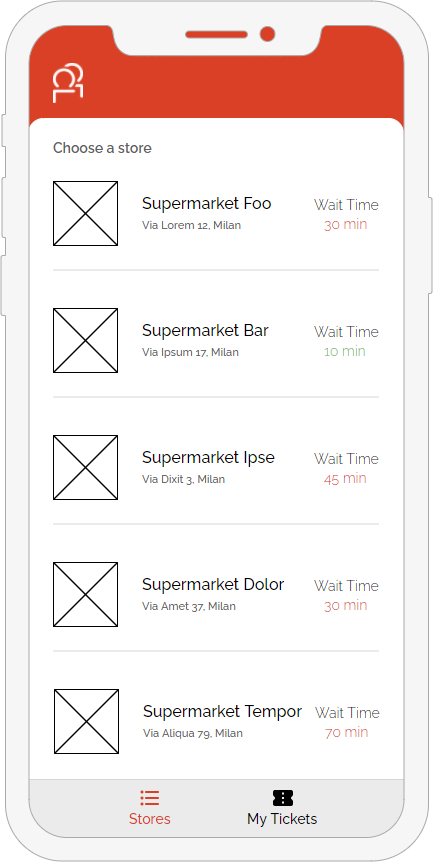
\includegraphics{home}
	\captionsetup{type=figure}
	\caption{App home.}
\end{minipage}%
\begin{minipage}{.5\textwidth}
	\centering
	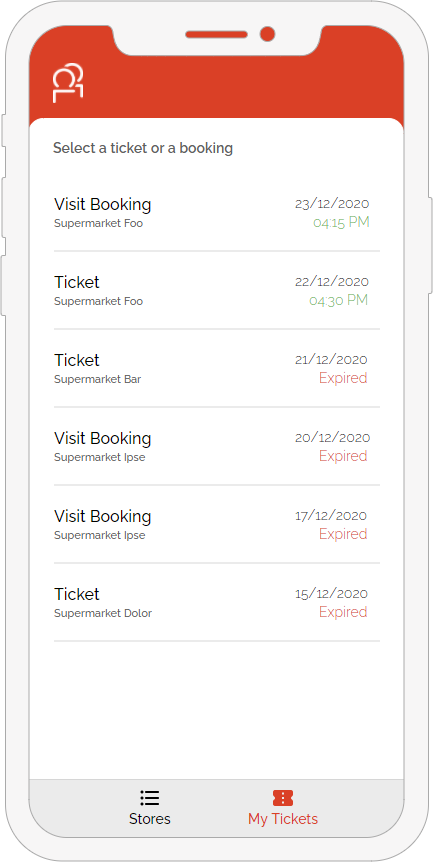
\includegraphics{my_tickets}
	\captionsetup{type=figure}
	\caption{Tickets list.}	
\end{minipage}

\clearpage

\begin{minipage}{.5\textwidth}
	\centering
	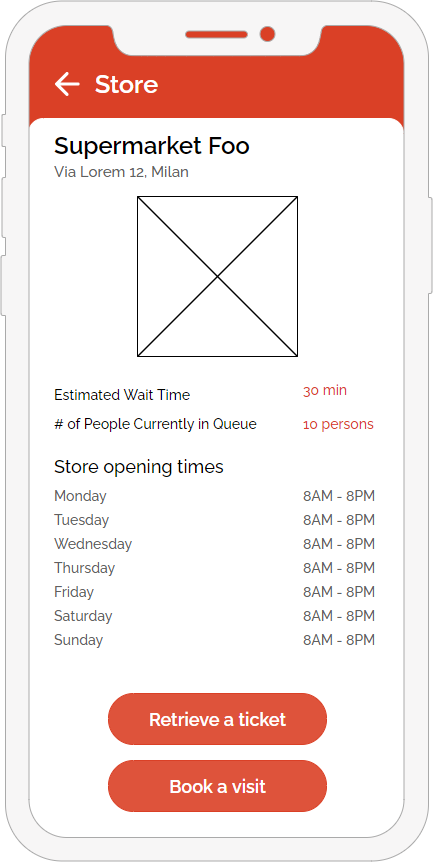
\includegraphics{store}
	\captionsetup{type=figure}
	\caption{Store page.}
\end{minipage}%
\begin{minipage}{.5\textwidth}
	\centering
	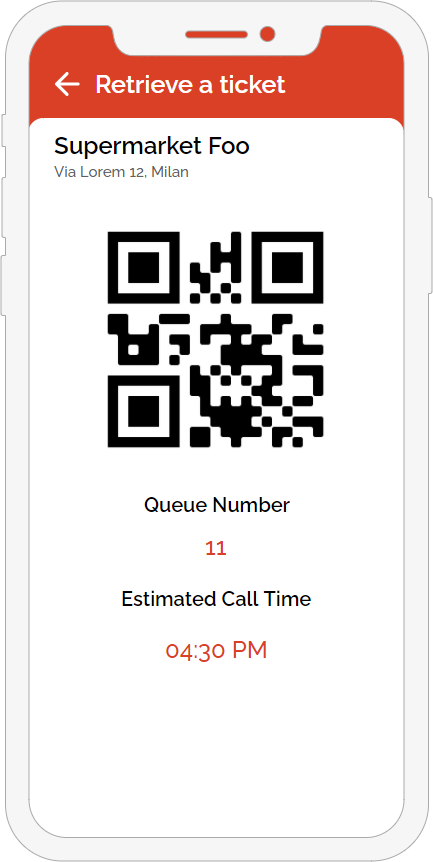
\includegraphics{ticket}
	\captionsetup{type=figure}
	\caption{Ticket Retrieved.}	
\end{minipage}

\vspace{2em}

\begin{minipage}{.5\textwidth}
	\centering
	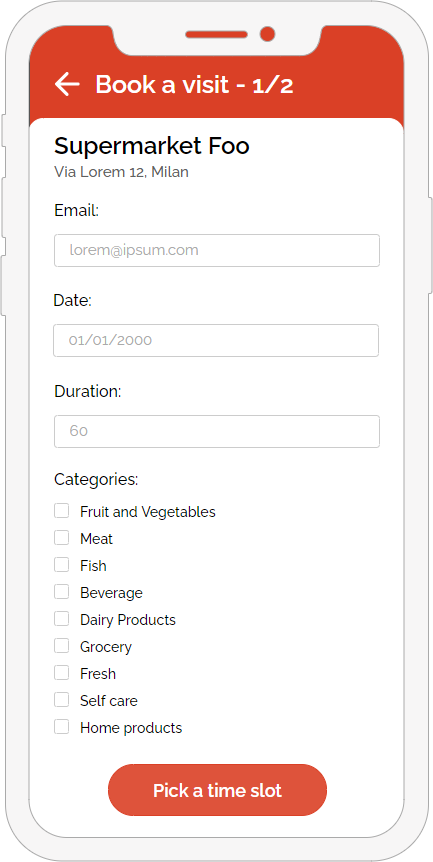
\includegraphics{book1}
	\captionsetup{type=figure}
	\caption{Book a visit (1/2).}
\end{minipage}%
\begin{minipage}{.5\textwidth}
	\centering
	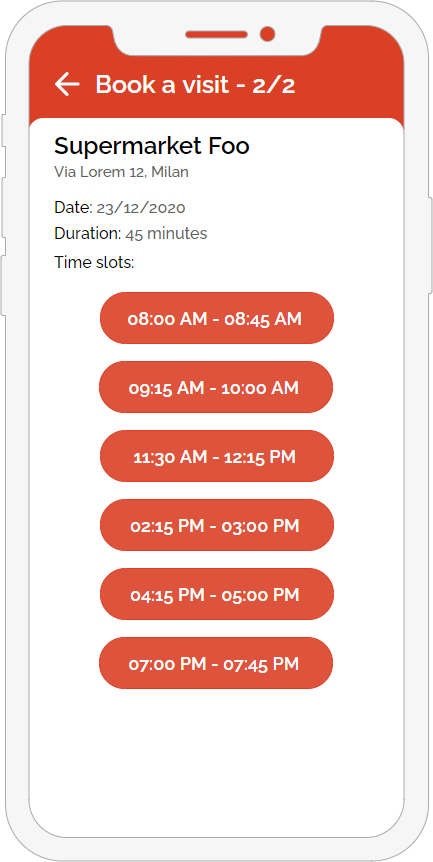
\includegraphics{book2}
	\captionsetup{type=figure}
	\caption{Book a visit (2/2).}	
\end{minipage}

\clearpage

\begin{figure}[H]
	\centering
	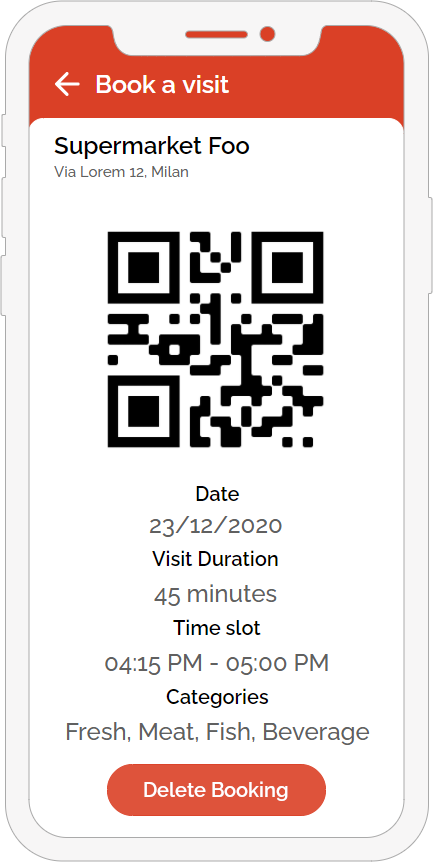
\includegraphics{book3}
	\caption{Visit booked.}	
\end{figure} 

Store managers and store employee use a web based interface for enjoying CLup features. The CLup admins can login at the same interface as well.
User interface mockups of most important pages of the web dashboard are shown below.
\vspace{2em}
\begin{figure}[H]
	\centering
	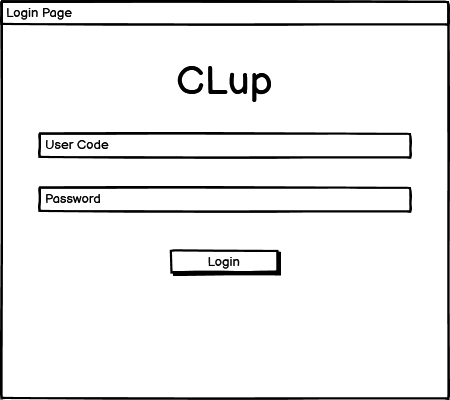
\includegraphics[width=0.77\linewidth]{login}
	\caption{Dashboard login.}	
\end{figure} 

\begin{figure}[H]
	\centering
	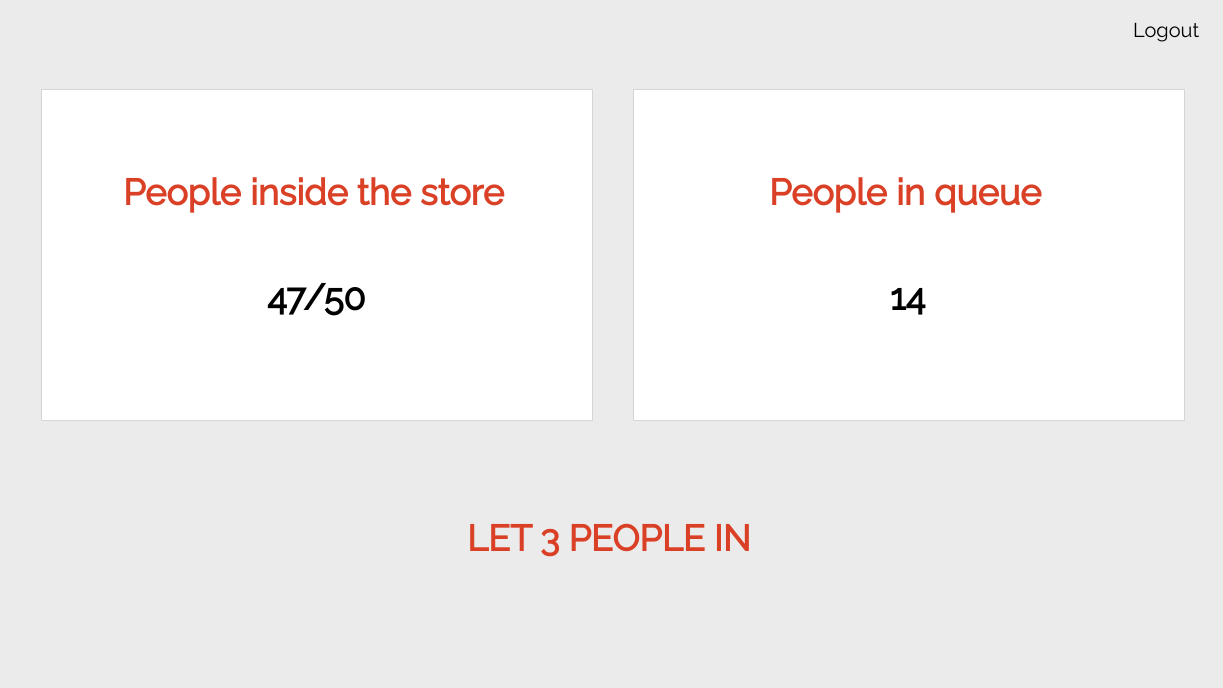
\includegraphics[width=0.77\linewidth]{employee}
	\caption{Employee homepage.}	
\end{figure} 
\begin{figure}[H]
	\centering
	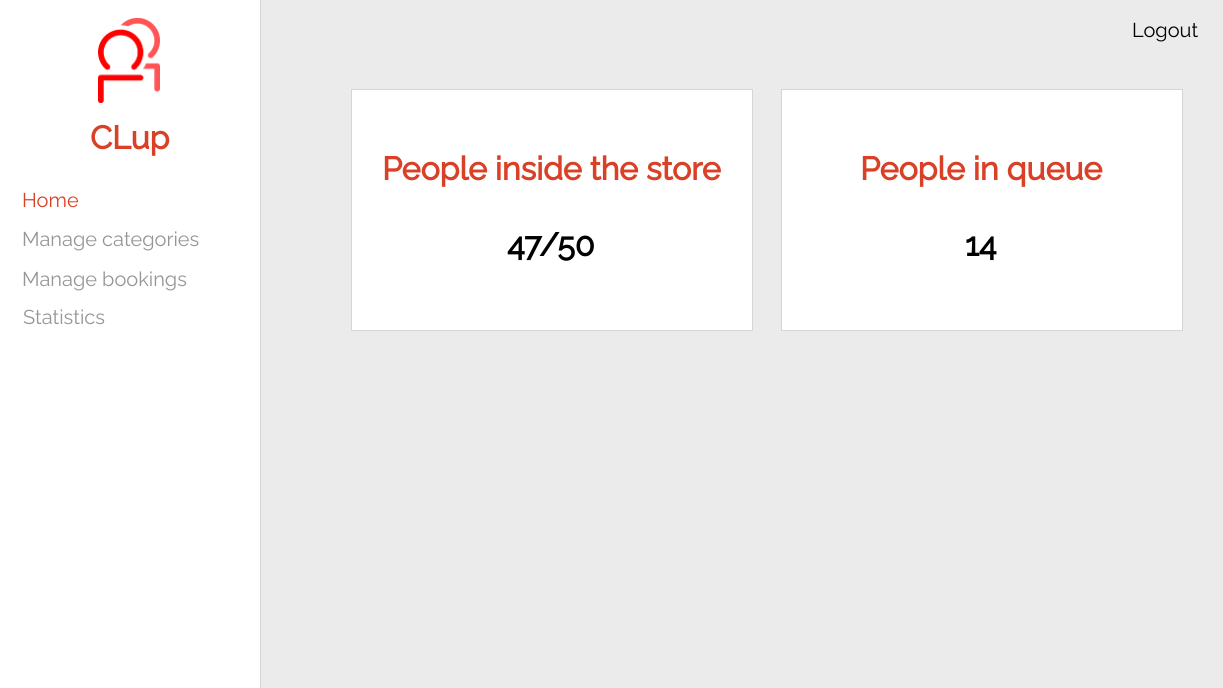
\includegraphics[width=0.77\linewidth]{dashboard1}
	\caption{Manager homepage.}	
\end{figure} 
\begin{figure}[H]
	\centering
	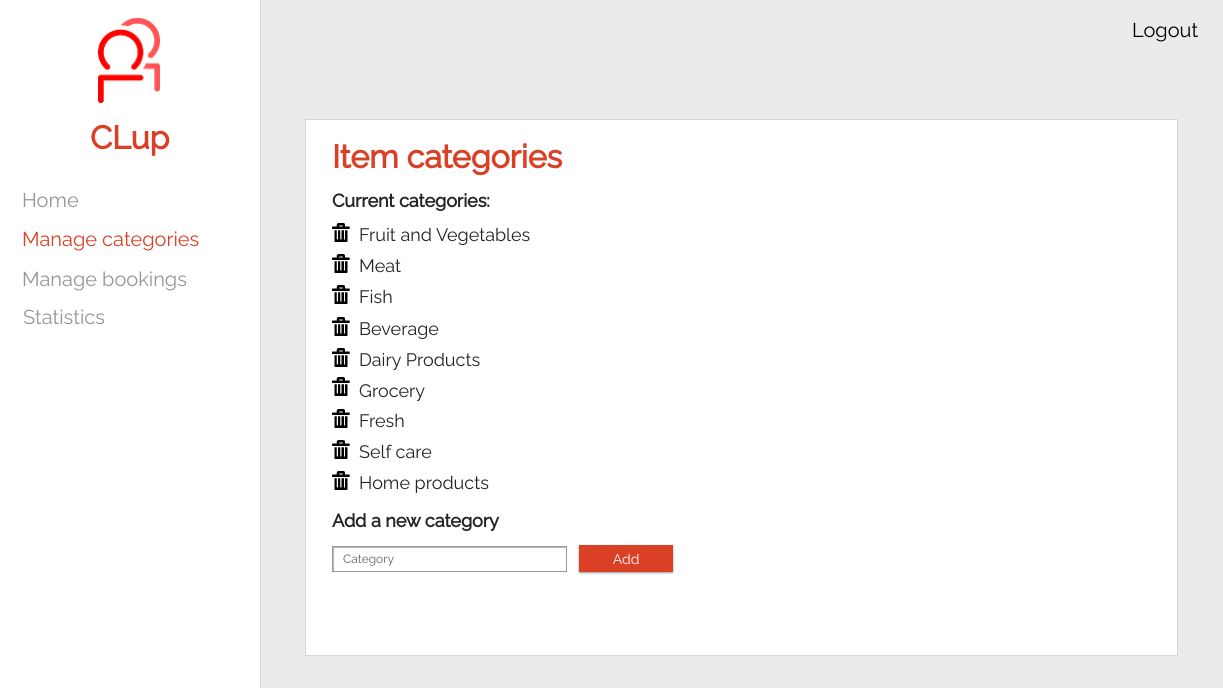
\includegraphics[width=0.77\linewidth]{dashboard2}
	\caption{Item categories page.}	
\end{figure} 
\begin{figure}[H]
	\centering
	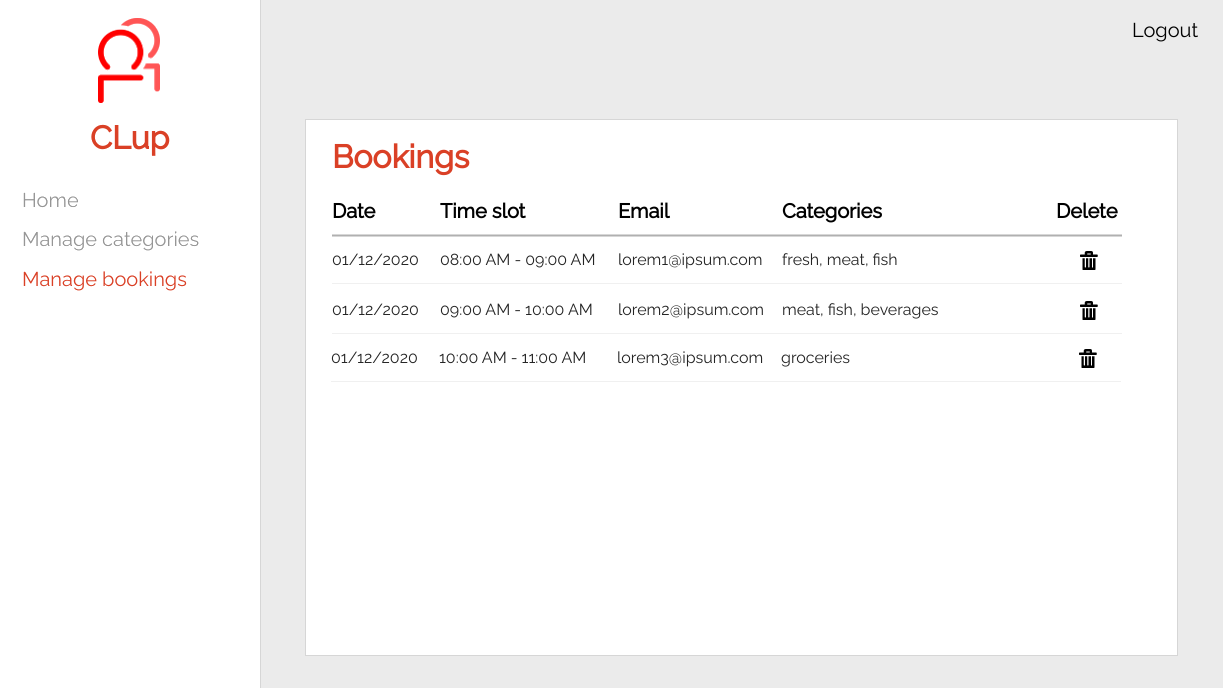
\includegraphics[width=0.77\linewidth]{dashboard3}
	\caption{Bookings list page.}	
\end{figure} 
\begin{figure}[H]
	\centering
	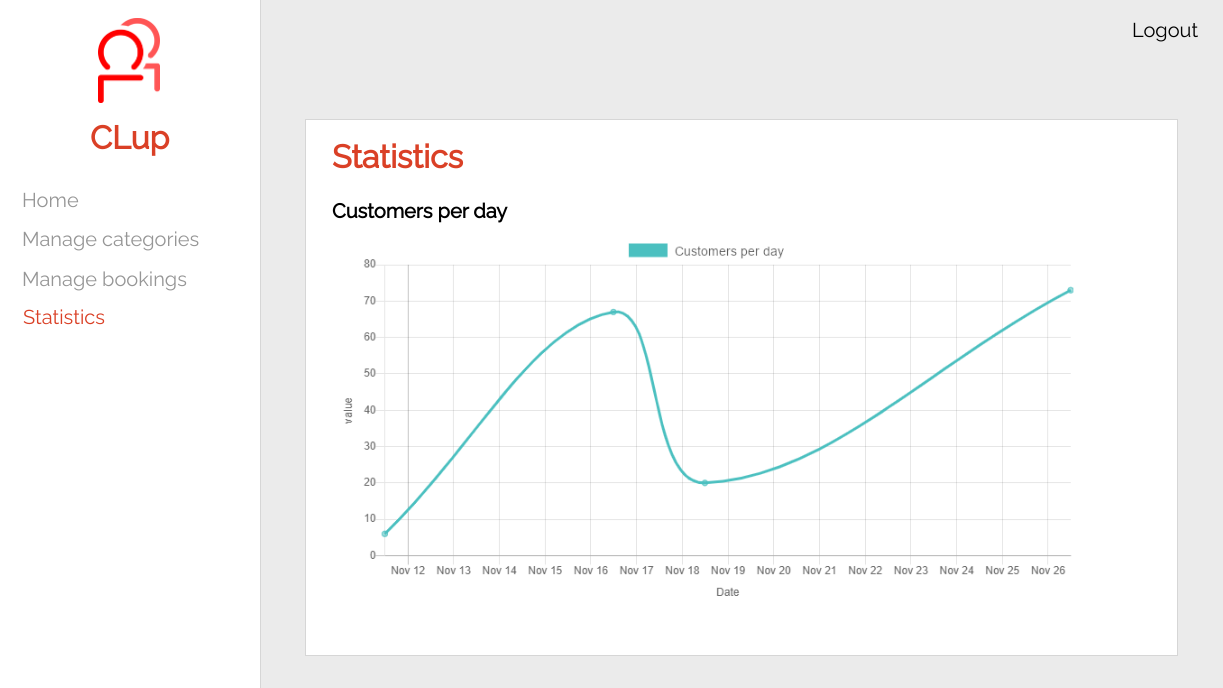
\includegraphics[width=0.77\linewidth]{dashboard4}
	\caption{Statistics page.}	
\end{figure} 
\begin{figure}[H]
	\centering
	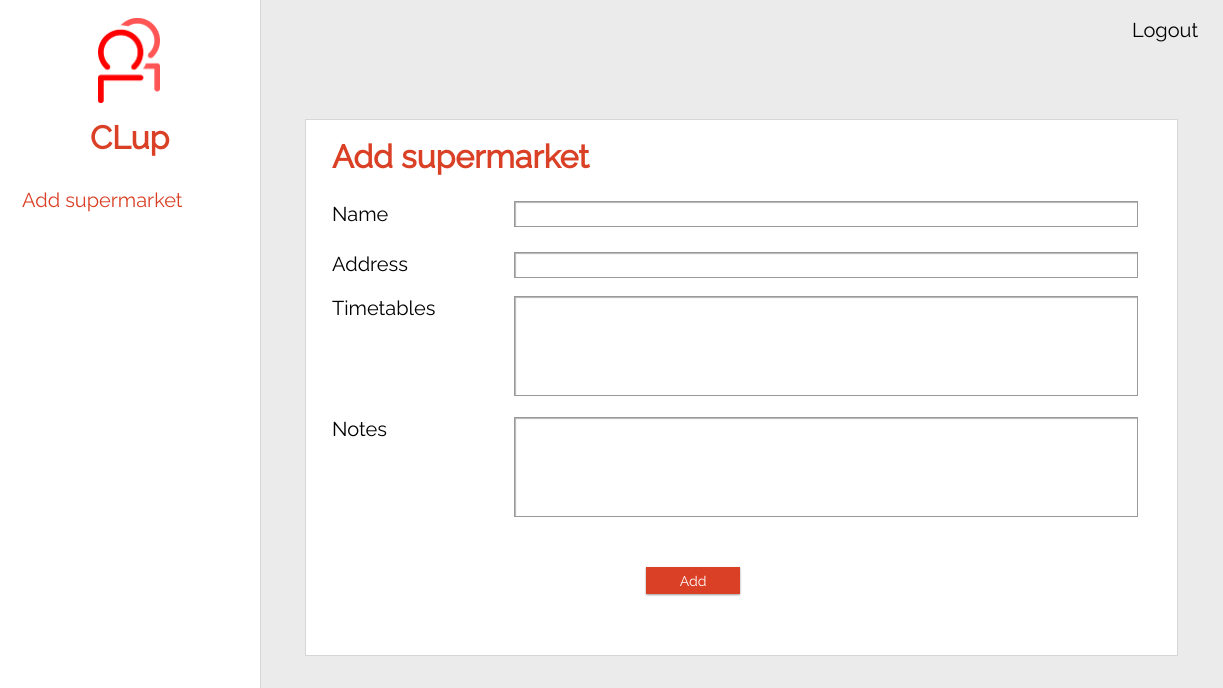
\includegraphics[width=0.77\linewidth]{new_store}
	\caption{Admin new supermarket page.}	
\end{figure} 
\clearpage

\subsection{Hardware Interfaces}
In addition to interfacing with computers (via a web browser), Clup interfaces with smartphones and their GPS module.
\subsection{Software Interfaces}
The system interfaces with a external map API for computing the distance between current place and store. It also permit to receive data
about QR codes via the public API.
\subsection{Communication Interfaces}
All the communications from and to CLup are made via HTTPS.

\section{Functional Requirements}
In this section, it is given a complete description of the functional requirements of the system.

    \subsection{Requirements}
    \subsubsection{Customers}
        \begin{enumerate}[label=\textbf{R.\arabic*}]
            \item
        \end{enumerate}

    \subsubsection{Store managers}
    \begin{enumerate}[label=\textbf{R.\arabic*}]
        \item
    \end{enumerate}

    \subsubsection{Store staff}
    \begin{enumerate}[label=\textbf{R.\arabic*}]
        \item
    \end{enumerate}

    \subsubsection{CLup admin}
    \begin{enumerate}[label=\textbf{R.\arabic*}]
        \item
    \end{enumerate}

    \subsection{Goal mapping on requirements}

    \subsection{Traceability matrix}

    \subsection{Scenarios}

    \subsection{Use cases description}
    % Use cases capture functional requirements of a system from the users' perspective.

\section{Performance Requirements}

\section{Design Constraints}

\section{Software System Attributes}